% Sección 10. Responsable: Juan Diego (#47).
% Cifras: outputs/modelado/interpretacion/ (scripts/modelado/interpretacion.py), generadas en el
% entorno de referencia (Docker, docs/REPRODUCIBILIDAD.md §1.1) con los modelos elegidos en #45.
\section{Interpretación}\label{sec:interpretacion}

La sección~\ref{sec:resultados} muestra que los cuatro modelos baten la barra. Esta sección pregunta \emph{en qué se apoyan} para hacerlo, y si eso coincide con las señales que encontró el análisis exploratorio (sección~\ref{sec:eda}): el día de la semana y el festivo. La pregunta es descriptiva. Una variable importante es una variable de la que el modelo depende para predecir, no una causa del hurto. Por ejemplo, que el modelo use el día anterior no significa que un día con muchos hurtos provoque otro al día siguiente. Toda cifra de esta sección sale de \texttt{outputs/\allowbreak{}modelado/\allowbreak{}interpretacion/}.

\subsection{Método: importancia por permutación agrupada}\label{sec:int-metodo}

Para los dos modelos de árboles, la importancia de una variable se mide como el aumento del MAE cuando se permutan sus valores entre los días \citep{breiman2001}. La permutación rompe la relación de esa variable con el número de víctimas y deja intactas las demás. Si el MAE no sube, el modelo no depende de ella.

Las 21 variables se agrupan en siete grupos, y las de cada grupo se permutan juntas. Muchas variables tienen sustitutas: el rezago de 7 días y el de 14 llevan casi la misma información. Si se permuta solo una, el modelo la suple con la otra y ambas parecen poco importantes. Al permutar el grupo entero, el modelo ya no tiene a qué recurrir.

La importancia se mide en dos sitios. El principal son los 184 días de evaluación, con el mismo modelo de la sección~\ref{sec:resultados}: reproduce su MAE de 32,72 y 34,22. El segundo son los seis pliegues de validación, con un modelo entrenado en cada uno. Si los dos coinciden, el resultado no depende de una ventana concreta. Cada grupo se permuta 50 veces en la evaluación y 25 en cada pliegue, con semilla fija. Nada de esto ajusta los modelos: las configuraciones son las elegidas en el ajuste de hiperparámetros.

SARIMA y ETS no tienen variables que permutar. Su estructura ya dice en qué se apoyan: en la propia serie, con una estacionalidad de periodo 7 y sin calendario. La sección~\ref{sec:int-series} lo retoma.

\subsection{En qué se apoyan los modelos de árboles}\label{sec:int-arboles}

La figura~\ref{fig:importancia} y la tabla~\ref{tab:importancia} muestran el resultado. Hay tres hallazgos.

\textbf{El ciclo semanal es la señal principal, y cada modelo la toma por un camino distinto.} El gradiente por histogramas la toma sobre todo del día de la semana: al permutarlo, su MAE sube un 35,0\,\%. El bosque aleatorio la toma sobre todo de los rezagos de 7, 14 y 28 días, que repiten lo ocurrido el mismo día de semanas anteriores, con un aumento del 26,3\,\%. Las dos vías llevan la misma información. Juntas confirman lo que el análisis exploratorio señaló como la señal más fuerte de la serie (sección~\ref{sec:eda-semana}).

\textbf{El día anterior importa tanto como el ciclo semanal.} El rezago de 1 día es el grupo más importante en la evaluación para los dos modelos: un 39,2\,\% y un 29,6\,\%. El análisis exploratorio no lo destacó como señal, pero sí lo anticipó la validación de los comparadores: el ingenuo, que repite el día anterior, gana en cuatro de los seis pliegues (sección~\ref{sec:barra}). Una lectura posible es que el rezago de 1 día recoge el nivel reciente de la serie. Ese nivel cambia de un año a otro (sección~\ref{sec:eda-anual}) y las variables de calendario no pueden darlo.

\textbf{Los festivos pesan aunque sean pocos.} Solo 8 de los 184 días de evaluación son festivos. Aun así, al permutar el grupo de festivos y puentes el MAE sube un 13,6\,\% y un 12,3\,\%. Casi todo ese peso está en la variable de festivo: el día anterior y el posterior a un festivo y el indicador de puente aportan menos del 0,5\,\% cada uno (\texttt{importancia\_\allowbreak{}variables\_\allowbreak{}evaluacion.csv}).

\begin{figure}[H]
\centering
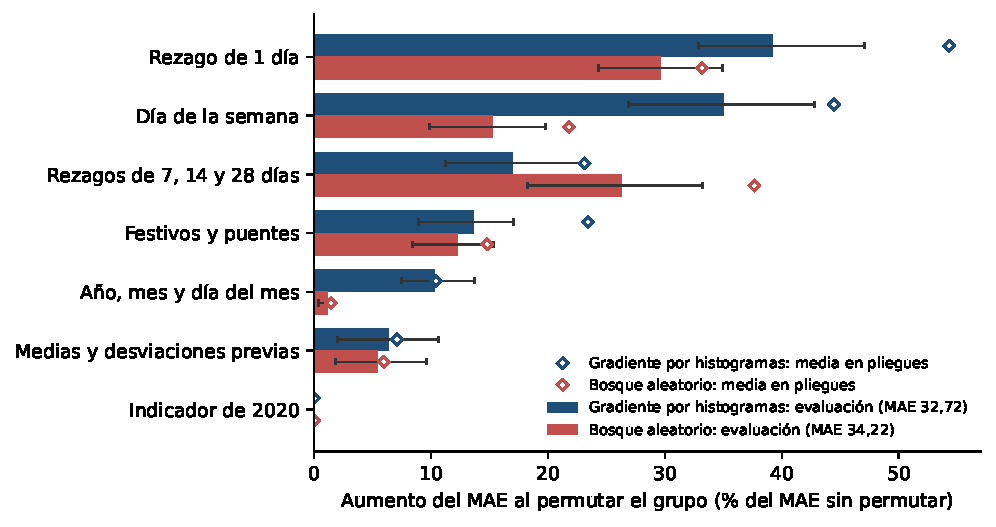
\includegraphics[width=0.92\textwidth]{figuras/importancia_permutacion_grupos.pdf}
\caption{Importancia por permutación agrupada de los dos modelos de árboles. Barras: aumento medio del MAE en los 184 días de evaluación al permutar cada grupo, con el intervalo entre los percentiles 5 y 95 de 50 permutaciones. Rombos: media de los seis pliegues de validación, con un modelo entrenado en cada uno. Fuente: \texttt{outputs/\allowbreak{}modelado/\allowbreak{}interpretacion/\allowbreak{}importancia\_\allowbreak{}grupos\_\allowbreak{}evaluacion.csv} e \texttt{importancia\_\allowbreak{}grupos\_\allowbreak{}pliegues.csv}.}\label{fig:importancia}
\end{figure}

\begin{table}[H]
\centering
\caption{Aumento del MAE al permutar cada grupo de variables, en porcentaje del MAE sin permutar. Evaluación: 184 días, 50 permutaciones. Pliegues: media de los seis pliegues de validación, con el mínimo y el máximo entre pliegues. Fuente: \texttt{outputs/\allowbreak{}modelado/\allowbreak{}interpretacion/\allowbreak{}importancia\_\allowbreak{}grupos\_\allowbreak{}evaluacion.csv} e \texttt{importancia\_\allowbreak{}grupos\_\allowbreak{}pliegues.csv}.}\label{tab:importancia}
\small
\setlength{\tabcolsep}{4pt}
\begin{tabular}{@{}lrlrl@{}}
\toprule
& \multicolumn{2}{c}{\textbf{Gradiente}} & \multicolumn{2}{c}{\textbf{Bosque aleatorio}} \\
\cmidrule(lr){2-3}\cmidrule(lr){4-5}
\textbf{Grupo} & \textbf{Evaluación} & \textbf{Pliegues} & \textbf{Evaluación} & \textbf{Pliegues} \\
\midrule
Rezago de 1 día & 39,2\,\% & 54,3 (44,7--81,5) & 29,6\,\% & 33,2 (27,5--40,2) \\
Día de la semana & 35,0\,\% & 44,5 (25,5--59,8) & 15,3\,\% & 21,8 (6,7--35,1) \\
Rezagos de 7, 14 y 28 días & 17,0\,\% & 23,1 (10,9--38,9) & 26,3\,\% & 37,6 (24,7--53,6) \\
Festivos y puentes & 13,6\,\% & 23,4 (16,8--31,6) & 12,3\,\% & 14,8 (9,8--20,2) \\
Año, mes y día del mes & 10,3\,\% & 10,4 (2,1--25,6) & 1,1\,\% & 1,4 ($-$0,2--4,2) \\
Medias y desviaciones previas & 6,3\,\% & 7,1 ($-$1,3--18,8) & 5,4\,\% & 5,9 (0,3--17,2) \\
Indicador de 2020 & 0,0\,\% & 0,0 & 0,0\,\% & 0,0 \\
\bottomrule
\end{tabular}
\end{table}

El orden se mantiene entre la evaluación y los pliegues. Salvo en el pliegue 5, los tres primeros grupos de cada modelo son los mismos en todos los pliegues. En el bosque aleatorio son los dos grupos de rezagos y el día de la semana. En el gradiente por histogramas son el rezago de 1 día, el día de la semana y, según el pliegue, los festivos o los rezagos semanales (\texttt{importancia\_\allowbreak{}grupos\_\allowbreak{}por\_\allowbreak{}pliegue.csv}). El pliegue 5 va de noviembre de 2024 a enero de 2025, la época en que el ciclo semanal se debilita (sección~\ref{sec:barra}). Allí el día de la semana baja al tercer puesto en el gradiente y al quinto en el bosque. En los pliegues las importancias son en general mayores que en la evaluación; no se investigó por qué.

Dos resultados piden cautela:
\begin{itemize}
\item \textbf{El indicador de 2020 da cero por construcción, no porque no importe.} En la evaluación y en los pliegues vale cero en todos los días, así que permutarlo no cambia nada. Lo mismo pasa con el año dentro de la evaluación, que es toda de 2025. El papel del indicador es otro: decide cómo usa el modelo los días de 2020 al entrenar, y eso se midió con la sensibilidad a 2020 de la sección~\ref{sec:res-sensibilidad}.
\item \textbf{El día del mes es una dependencia que el análisis exploratorio no explica.} En el gradiente por histogramas, permutar solo el día del mes sube el MAE un 8,6\,\%; en el bosque aleatorio, un 0,9\,\%. El análisis exploratorio estudió el mes (sección~\ref{sec:eda-mes}), pero no el día del mes. Como el grupo de año, mes y día del mes varía entre el 2,1 y el 25,6\,\% según el pliegue, esta dependencia puede reflejar fechas concretas del entrenamiento más que un patrón estable. No se interpreta sin un análisis específico.
\end{itemize}

\subsection{Contraste con el análisis exploratorio}\label{sec:int-eda}

La importancia dice que el modelo usa una variable, pero no si la usa en el sentido que mostró el análisis exploratorio. Para comprobarlo se comparan dos magnitudes (tabla~\ref{tab:contraste-eda}).

\textbf{El perfil semanal.} En la evaluación, el viernes registra un 42,5\,\% más de víctimas que el domingo. Es menos que el 65\,\% de la serie completa porque, en la evaluación, el domingo está un 24\,\% por encima de su media histórica (302,9 frente a 245,0) y el viernes solo un 7\,\% (431,6 frente a 403,1) (\texttt{perfil\_\allowbreak{}semanal\_\allowbreak{}evaluacion.csv}). Los modelos siguen la diferencia de la evaluación y no la histórica: dan un 47,3\,\% y un 39,7\,\%. El ciclo semanal que aprendieron no es un patrón fijo. Una explicación compatible con la sección~\ref{sec:int-arboles}, aunque no se comprobó, es que se ajusta al nivel reciente a través de los rezagos.

\textbf{El festivo.} Se toman los lunes del entrenamiento sin días faltantes en los rezagos y se cambia solo el indicador: los laborables se marcan como festivos y los festivos como laborables, con todo lo demás igual. Al marcar un lunes laborable como festivo, el gradiente por histogramas baja su pronóstico un 37,3\,\% y el bosque aleatorio un 30,2\,\%. El análisis exploratorio midió una diferencia del 37,8\,\% entre los lunes festivos y los laborables (tabla~\ref{tab:eda-festivos}). El gradiente reproduce casi exactamente esa magnitud, y el bosque la reproduce en parte. Este cambio es la respuesta del modelo a su variable, no el efecto causal de un festivo: el ejercicio no altera lo que acompaña a un festivo real, como el día anterior o el puente.

\begin{table}[H]
\centering
\caption{Señales del análisis exploratorio frente a lo que reproducen los modelos de árboles. Perfil semanal: media diaria del viernes sobre la del domingo, menos uno, en los 184 días de evaluación. Festivo: cambio del pronóstico al marcar como festivos los lunes laborables del entrenamiento (218 lunes), con lo demás fijo. Fuentes: \texttt{outputs/\allowbreak{}eda/\allowbreak{}resumen\_\allowbreak{}eda.json}, \texttt{outputs/\allowbreak{}modelado/\allowbreak{}interpretacion/\allowbreak{}resumen\_\allowbreak{}interpretacion.json}.}\label{tab:contraste-eda}
\small
\begin{tabular}{@{}lrrrr@{}}
\toprule
\textbf{Señal} & \textbf{EDA (2020--2025)} & \textbf{Observado} & \textbf{Gradiente} & \textbf{Bosque} \\
\midrule
Viernes frente a domingo & 65\,\% & 42,5\,\% & 47,3\,\% & 39,7\,\% \\
Lunes festivo frente a laborable & $-$37,8\,\% & --- & $-$37,3\,\% & $-$30,2\,\% \\
\bottomrule
\end{tabular}
\end{table}

\subsection{SARIMA y ETS: lo que su estructura no ve}\label{sec:int-series}

SARIMA y ETS modelan el ciclo semanal de forma explícita, con una estacionalidad de periodo 7, y el nivel reciente con su componente de nivel o sus términos autorregresivos. Así cubren las dos señales principales de los árboles, lo que es coherente con que su MAE sea similar (tabla~\ref{tab:resultados}). Lo que no tienen es calendario. Pronostican un festivo como un día normal de su día de la semana, y sobrestiman los ocho festivos de la evaluación en entre 56 y 59 víctimas de media (tabla~\ref{tab:festivos}). Es la señal del análisis exploratorio que los árboles usan y estos modelos no.

\subsection{Síntesis}\label{sec:int-sintesis}

Los modelos se apoyan en las señales que anticipó el análisis exploratorio. El ciclo semanal es la principal, y el gradiente lo toma del día de la semana y el bosque de los rezagos semanales. El festivo aparece con una magnitud parecida a la medida en el análisis exploratorio. A eso se suma una señal que el análisis exploratorio no destacó y que la validación de los comparadores sí anticipaba: el nivel del día anterior. Ninguna de estas importancias es causal. Describen de qué información depende el pronóstico, no qué produce el hurto. La dependencia del gradiente respecto al día del mes queda como un patrón sin explicar.
